\section{Periodiska systemet}
\vfill
\begin{figure}[h!]
    \centering

    \makebox[\textwidth]{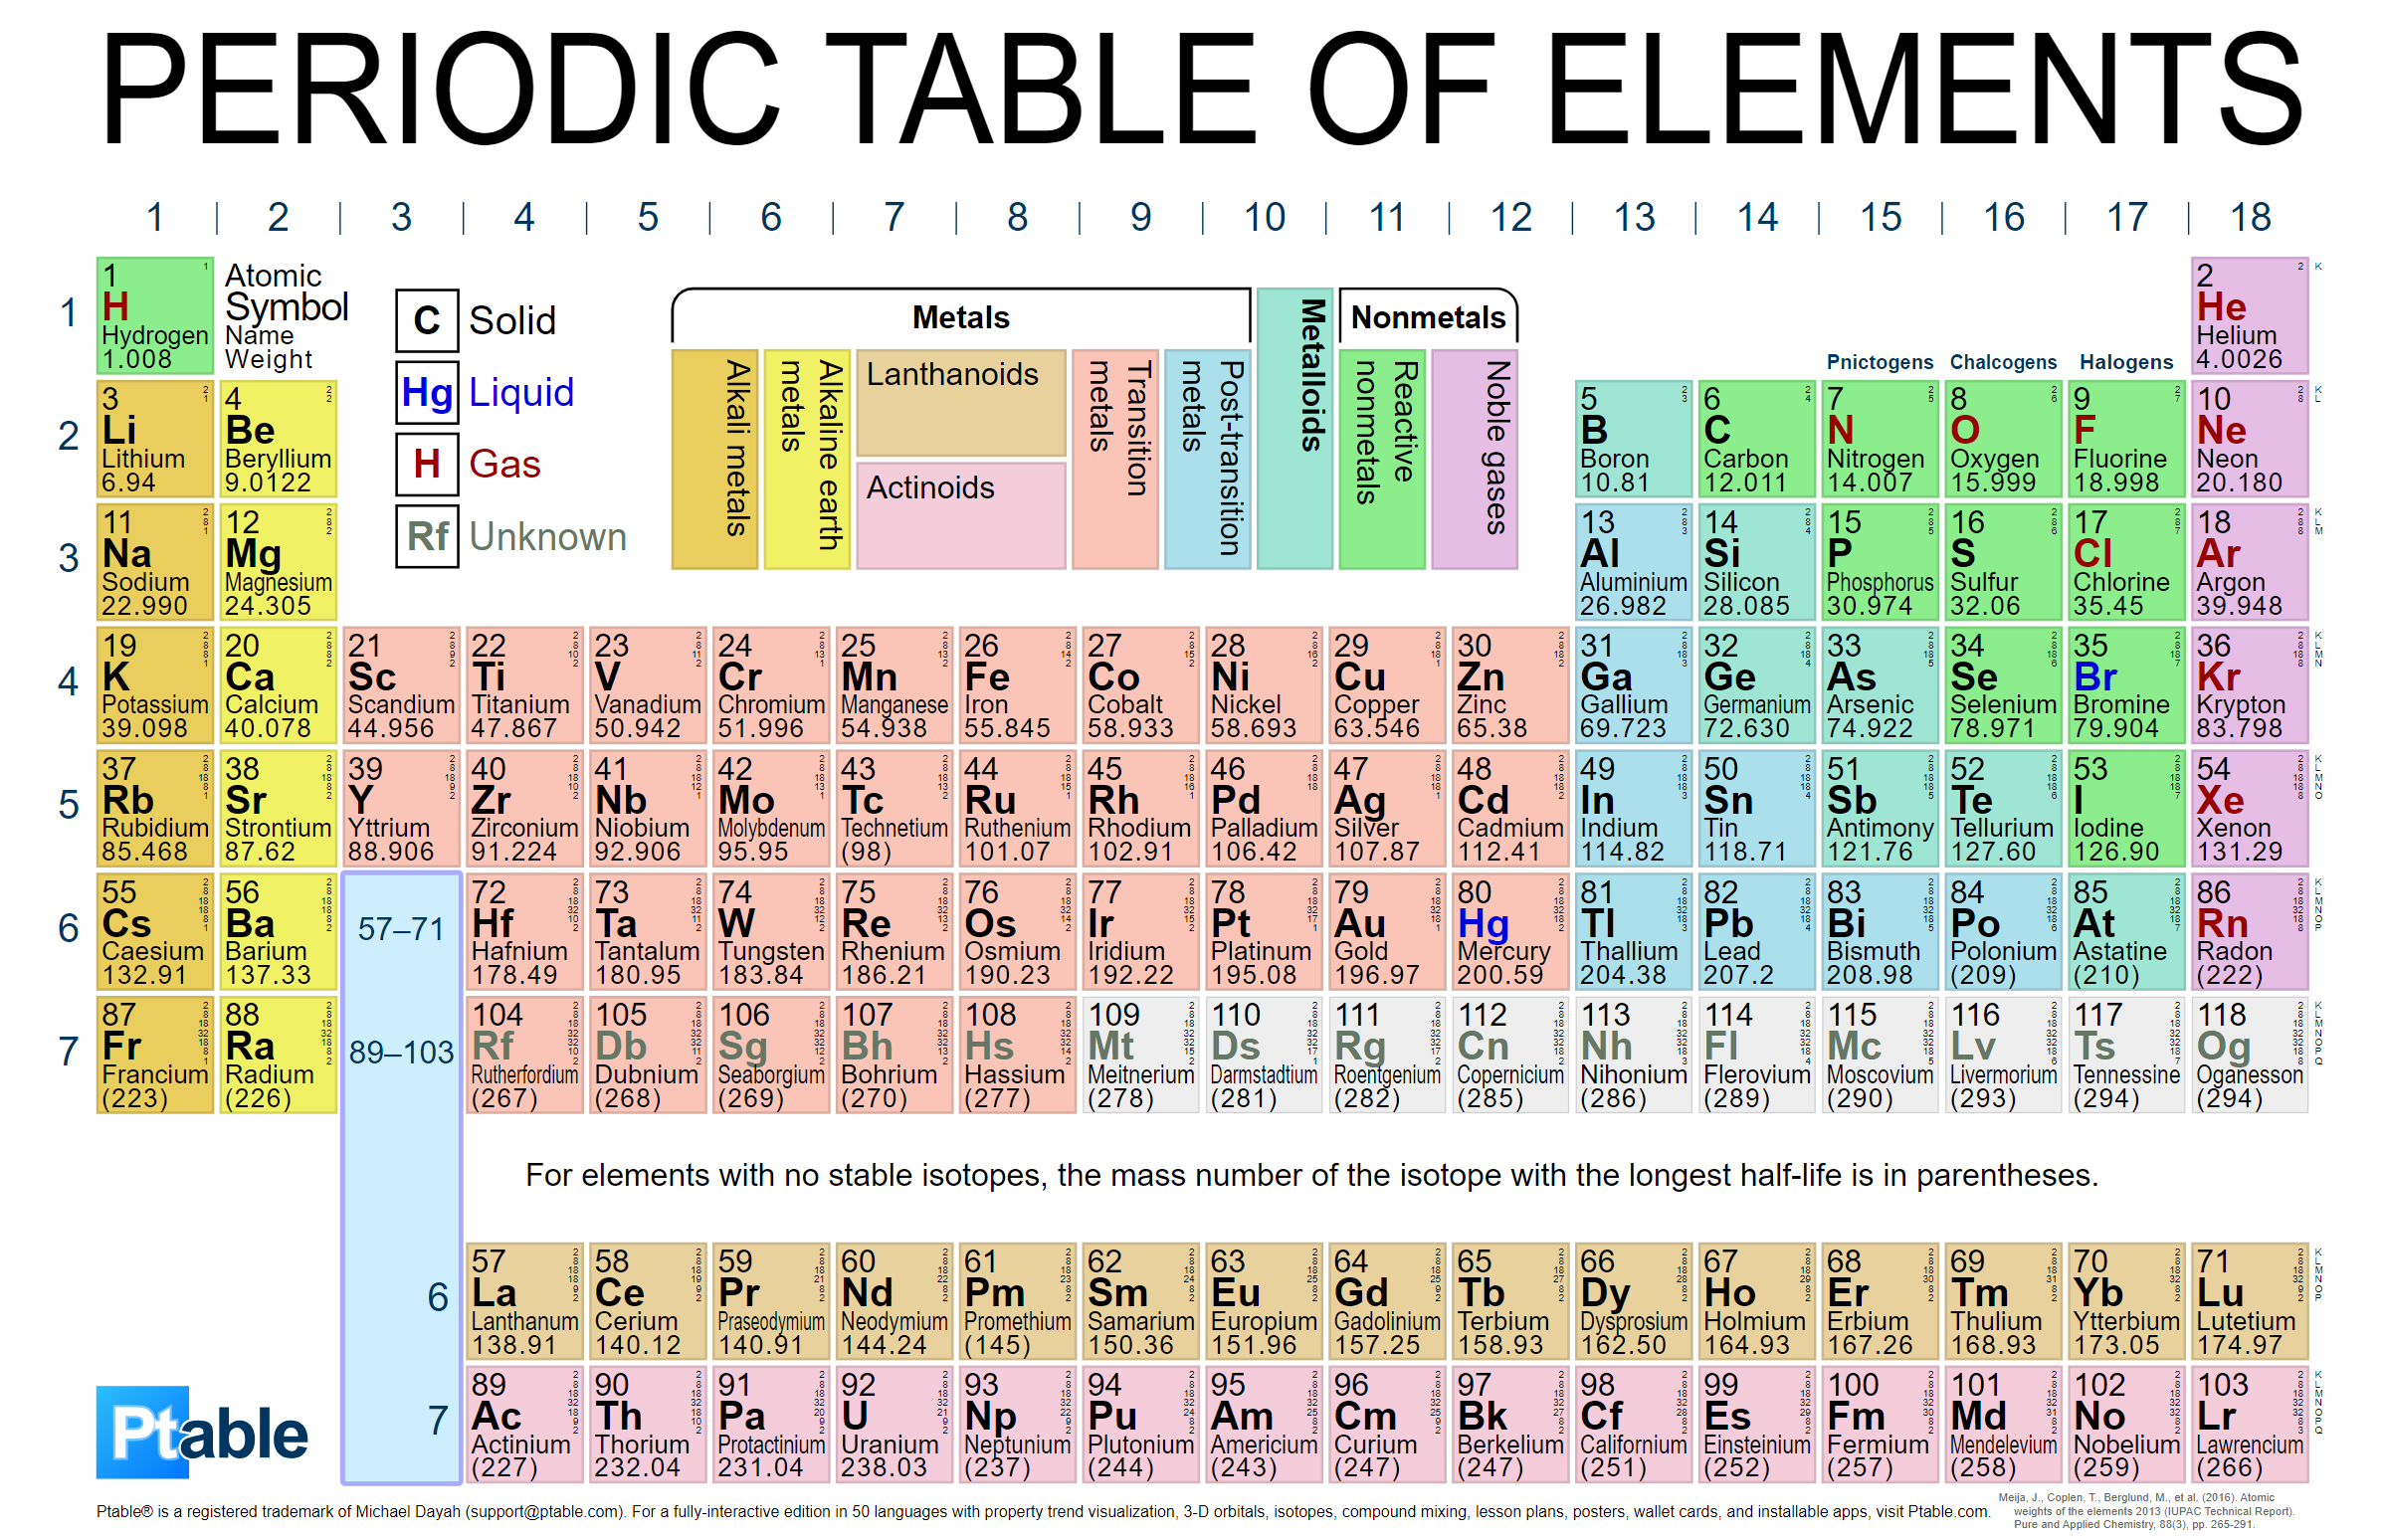
\includegraphics[angle=90,origin=c,width=.629\paperwidth]{img/periodic-table.png}}
    \caption{Periodiska systemet.}
\end{figure}
\vfill
\pagebreak

\section{Formelsamling}

\subsection{Konstanter}
\begin{tabular}{c | c}
    \textbf{Konstant} & \textbf{Värde} \\ \toprule
    $\pi$ & \num{3.14159265359} \\
    $c$ & \SI{299792458}{\m\per\s} \\

\end{tabular}